\chapter{Conceito do Sistema}
\label{chap:concep}
%durante todo o desnvolvimento do capítulo vc usa o termo futuro nos verbos, vc precisa utilizar o presente, vcs já realizaram isso.

\begin{flushright}
   \begin{list}{}{
      \setlength{\leftmargin}{4.5cm}
      \setlength{\rightmargin}{0cm}
      \setlength{\labelwidth}{0pt}
      \setlength{\labelsep}{\leftmargin}}
      \item Para um robô, o ambiente é um mar de ambiguidades, no qual ele vai afundar ou nadar a depender da robustez de sua percepção.
      \begin{list}{}{
      \setlength{\leftmargin}{0cm}
      \setlength{\rightmargin}{0cm}
      \setlength{\labelwidth}{0pt}
      \setlength{\labelsep}{\leftmargin}}
      \item \cite{Fitzpatrick}
      \end{list}
   \end{list}
\end{flushright}

A percepção é, de acordo com o dicionário \citeonline{perc_michaelis}, a capacidade de distinguir por meio dos sentidos ou da mente.

Segundo \citeonline{chuck}, este é o ponto fraco mais comum em robôs pois para garantir sua segurança e confiabilidade é necessário que o mesmo tenha a capacidade de interpretar as variáveis ambientais. A percepção é o que torna os robôs diferentes de simples mecanismos, pois é ela quem dá a habilidade de adequar suas operações de acordo com as influências externas.

A percepção do ELIR pode ser definida como um sistema integrado de sensoriamento e com unidades de processamento, em que seus dados serão utilizados como parâmetros de tomada de decisão e disponibilizados durante a operação de inspeção ao operador.
%este parágrafo está um pouco confuso, parece que vc não quer falar do outro sistema. o de movimentação. retrabalhe ele e reforce que vc irá entregar os dados para um outro sistema de movimentação.

A Percepção é o sistema de sensoriamento do robô e pode ser entendida como a forma que ele compreende o que esta ao seu redor. No projeto do robô ELIR, o sistema de percepção engloba a aquisição e a interpretação dos dados de todos os sensores envolvidos. Para isso, foi escolhido o \textit{framework} de robótica ROS como ambiente de trabalho do projeto.
%da forma como apresentada, a escolha do ROS foi por causa da Percepção, e isso não é verdade.

Segundo a \citeonline{ROS}, o ROS é um ambiente flexível para desenvolvimento de \textit{software} para robótica. O \textit{framework} possui uma coleção de ferramentas, bibliotecas e convenções que simplificam tarefas de criação de comportamentos complexos para robôs. A escolha foi feita com base em suas funcionalidades, pois usando o ROS é possível ter uma arquitetura de processamento de dados em quase em paralelo.

\citeonline{Alvaro} diz que o ROS é composto por um conjunto de atributos, porém os que têm uma importância mais relevante em um aprendizado rápido de como utilizar a plataforma, são os nós ou \textit{Nodes} e os pacotes ou \textit{Packages}. Os nós são estruturas que possuem algumas funções ou métodos dentro. %algumas funções dentro??? explique
Eles compõem uma estrutura maior que são os pacotes, este pode ser visto como uma funcionalidade completa como um conjunto de classes que formam um sistema, ou seja, seria como falar dos módulos de um programa.

Cada nó pode se comunicar com outro de duas maneiras: através de um tópico ou de um serviço.

 Um tópico é basicamente um canal, como um espaço de memória, no qual os nós trocam mensagens. Tais mensagens são trocadas de forma anônima, ou seja, em geral os nós não sabem com quem estão se comunicando. Os dados podem ser enviados e lidos de um tópico através de uma publicação e uma subscrição respectivamente.

A estrutura de tópicos é bastante flexível em questões de comunicação, porém uma comunicação de muitos-para-muitos não é adequada para mensagens de requisição. %aqui faltou uma concatenação para vc vier e poder falar dos serviços
Os serviços foram criados como um par de mensagem que possui uma requisição e uma resposta. Geralmente são usados para solicitação de dados específicos ou em funcionalidades de emergência. Na figura \ref{Fig:ros}, pode-se observar um esquemático representando a estrutura básica do ROS.

\begin{figure}[!ht]
\centering
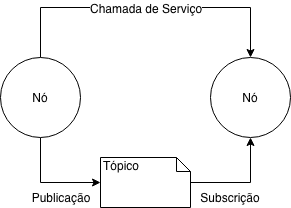
\includegraphics[width=10cm]{Figures/ros.png}
\caption{Estrutura básica do ROS}\label{Fig:ros}
\caption*{Fonte: ????}
\end{figure}

O sistema foi projetado de forma a possuir três subsistemas principais: aquisição, localização e detecção, com objetivo de cumprir os requisitos impostos pelo cliente.

\section{Especificação técnica do sistema de Percepção}
\label{ssec:espt}

%elaborar um parágrafo introdutório para a especificação
O desenvolvimento do conceito do sistema de Percepção teve como base os requisitos técnicos do cliente e as especificações podem ser observadas abaixo:
\begin{itemize}
\item O sistema foi projetado para trabalhar com alimentação de 14V proveniente de baterias LiPo.
\item A máxima temperatura de trabalho na \textit{housing} é de 50 graus Celsius.
\item O sistema consegue detectar objetos através do sonar em uma faixa de servidão de 6.45 metros.
\item A obtenção de \textit{frames} da câmera IR acontece na taxa de 1 frame a cada dois segundos.
\item Em condições de sobretemperatura ou sobrecorrente o sistema alertará o operador.
\item O sistema não é protegido contra ingresso de água
\end{itemize} 

\section{Arquitetura geral do sistema de Percepção}
\label{ssec:arqg}
%a arquitetura não é apra simplificar o projeto, é um instturmento usado para organizar as ideias e implementar um certe planejamernot no desenvolvimeto
Para simplificar o sistema como um todo, foi elaborado um esquemático representando o projeto conceitual da arquitetura geral do sistema, mostrado na Fig. \ref{arqgeral}. Nela estão representados as três camadas principais: \textit{Sensing}, \textit{Interface} e \textit{ROS Environment}.

\begin{figure}[!ht]
\centering
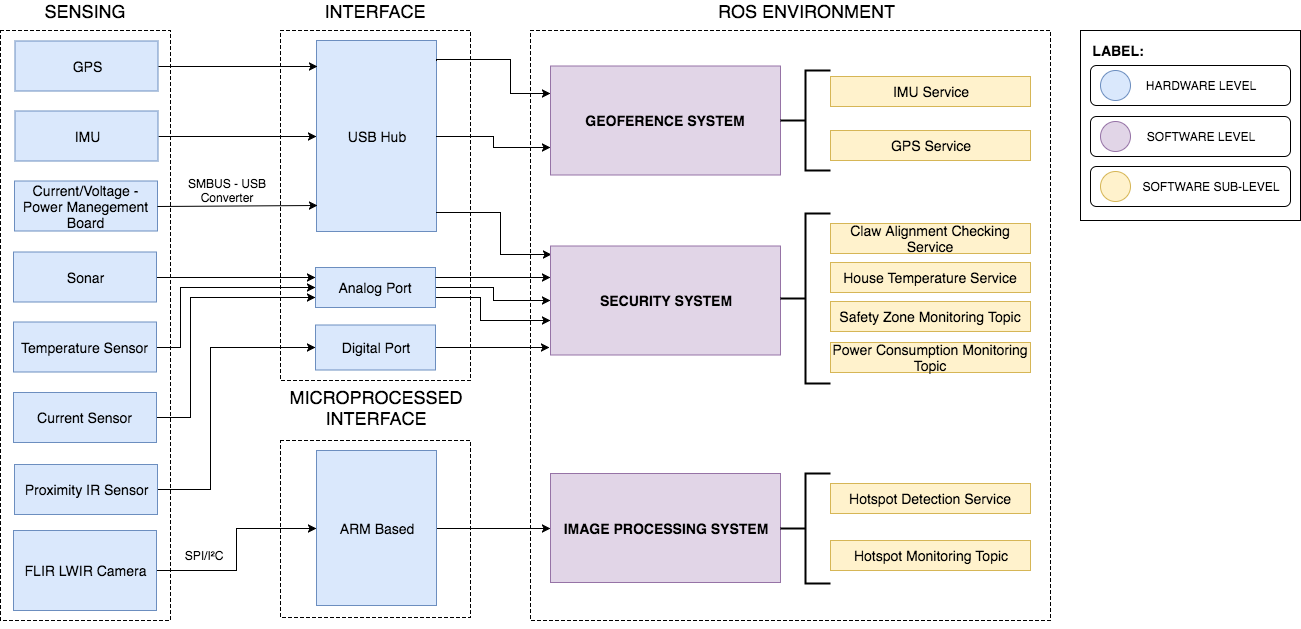
\includegraphics[width=15cm]{Figures/ArquiteturaPerceptionv2.png}
\caption{Arquitetura Geral da Perception}\label{arqgeral}
\caption*{Fonte: os autores}
\end{figure}

%não entendi, vc estava chamando de camadas e agora são etapas????
 A etapa de \textit{Sensing} é uma camada de \textit{hardware} composta por todos os processos de aquisição de dados de todos os sensores envolvidos no projeto. É nela em que todas as variáveis do ambiente que o sistema solicita são coletadas.
 
Os sensores GPS e IMU são responsáveis por coletar os dados de georreferenciamento e de inclinação do robô. O primeiro será usado para informar ao final da missão as coordenadas em que foi detectado um ponto quente na linha de transmissão. O segundo é utilizado para verificar se o robô está com alguma inclinação no cabo para dar inicio a algum movimento.

O sonar e a câmera térmica fazem parte do subsistema de detecção de objetos dentro da linha de servidão e de pontos quentes respectivamente. A partir da detecção de algum desses eventos, será armazenado a localização e a imagem do local onde ocorreu. 

Os sensores de proximidade IR verificam se as garras do robô estão alinhadas com o cabo antes de realizar alguma atuação. As garras estão representadas pelo número 4 no primeiro esquemático mecânico do Apêndice \ref{Append:diagmec}.

O \textit{Smart Charger} e os sensores de corrente são responsáveis por adquirir os dados de consumo do robô. Com o \textit{Smart Charger} é possível adquirir dados de temperatura, corrente, tensão e capacidade das baterias. O sensores de corrente coletam informação de cada conjunto de motor, como pode ser visto no esquemático eletrônico no Apêndice \ref{Append:diagele}.

E por final, tem-se o sensor de temperatura que monitora se há aquecimento dentro da casa de eletrônicos do robô.
  
A etapa \textit{Interface} é composta por camadas de \textit{hardware} e \textit{firmware}, que são responsável por transmitir os dados coletados dos sensores para o ambiente de trabalho ROS.

Nela, tem-se três interfaces de comunicação: 

\begin{itemize}
	\item a \textit{Phidgets}, representada por "Interface" na Figura \ref{arqgeral}. Responsável por coletar os dados dos sensores digitais, analógicos e USB.
	\item um microcontrolador STM32F401RE, para adquirir os dados da câmera térmica via protocolo VoSPI.
	\item um microcontrolador STM32L432KC, para adquirir os dados do \textit{Smart Charger} via protocolo SMBus.
\end{itemize}
 
 
 Por último, terá a camada de \textit{software}, a qual será feita no ambiente ROS, e que irá englobar todo o sistema de compreensão e interpretação dos dados provenientes do sistema de interfaceamento do robô. Nela também está contida uma interface gráfica para interação com o usuário, que servirá como meio de supervisório para os dados mais importantes do robô. O \textit{layout} conceitual da UI pode ser vista no Apêndice \ref{Append:wireframes}. 
 
 As funcionalidades do sistema de percepção serão melhor abordadas na seção \ref{chap:mat}.
 
% \pagebreak

\section{Arquitetura de software do sistema de Percepção}
\label{ssec:arqsp}


A arquitetura de software foi projetada em três camadas a fim de facilitar o desenvolvimento do sistema e simplificar o entendimento do mesmo. As camadas são:

\begin{itemize}
	\item \textit{User Interface Layer}
	\item \textit{Business Layer}
	\item \textit{Drvier Layer}
\end{itemize}
 
As camadas e seus componentes podem ser vistos na Fig.\ref{arqsoft}.

\begin{figure}[h]
	\centering
	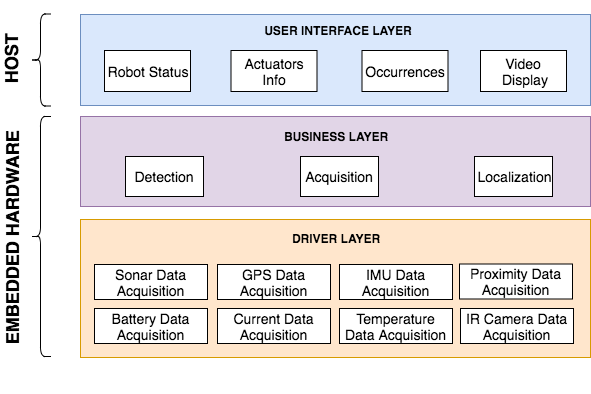
\includegraphics[width=15cm]{Figures/ArquiteturadeSoftware.png}
	\caption{Arquitetura Geral da Perception}
	\caption*{Fonte: os autores.}
	\label{arqsoft}
\end{figure}

\subsection{Driver Layer}
	
A camada de \textit{Driver Layer} está diretamente relacionada a funcionalidade de aquisição de dados. Ela composta pelo \textit{hardware}, representado pelos sensores e seus respectivos drivers de comunicação. Desta forma, as subcamadas são nomeadas com o processo de aquisição de dados de cada sensor envolvido no projeto.

%não entendo isso como subcamadas. chame por um outro nome e não subcamandas, para mim elas são como processos de uma camada
As subcamadas \textit{Current Data Acquisition}, \textit{Temperatura Data Acquisition}, \textit{Proximity Data Acquisition} e \textit{Sonar Data Acquisition} são responsáveis por adquirir as informações analógicas de seus sensores e transformá-los em dados da grandeza física a ser medida. Todas estas subcamadas utilizam a placa de interfaceamento Phidgets para o estabeler de comunicação entre o computador (NUC) e os sensores.

As subcamadas \textit{IMU Data Acquisition} e \textit{GPS Data Acquisition} são responsáveis pelo recebimento de dados da IMU e do GPS seguindo o protocolo de comunicação do fabricante. Esses dois módulos estão conectados ao \textit{hub} USB da placa de interfaceamento Phidgets. 

A subcamada de \textit{IR Camera Data Acquisition} é responsável pela aquisição de dados da câmera térmica, a qual se comunica via VoSPI com um microcontrolador de arquitetura ARM (STM32F401RE) e converte os dados para USB e os envia à NUC. 

Por último, a subcamada de \textit{Battery Data Acquisition} é responsável pelo estabelecimento da comunicação e coleta de informações com o \textit{Smart Charger} de bateria utilizando protocolo SMBus.

As conexões e diagramas elétricos podem ser vistos no apêndice \ref{Append:diagele}.

\subsection{Business Layer}

A camada \textit{business layer} é responsável por implementar a regra de negócio do sistema. As funcionalidades do sistema são representadas como sub-camadas da business layer, pois são elas responsáveis pelo processamento e coordenação dos dados adquiridos pela camada de aquisição.

\subsection{User Interface Layer}

A camada de \textit{User Interface} foi projetada para disponibilizar os dados para o operador. Nela será mostrado de forma resumida os dados mais relevantes do robô e da operação. Nesta camada existem três subcamadas: \textit{Robot Status Display, Actuators Display} e \textit{Video Display}. 

A subcamada \textit{Robot Status Display} disponibiliza os dados de integridade do robô como temperatura, corrente, tensão, nível de bateria, entre outras informações. A subcamada de \textit{Actuators Display} disponibiliza o dados de todos os motores do robô, como carga, temperatura, status e corrente. Por último, a subcamada de \textit{Video Display} mostra em tempo real o monitoramento realizado pela câmera térmica, possibilitando o usuário ver os componentes da linha que estão com temperatura elevada e até mesmo identificar pontos quentes.

A interface irá se resumir em duas telas: A tela principal com um layout de \textit{dashboard}, e outra que terá as informações dos atuadores. O \textit{dashboard} será um painel de monitoramento, no qual haverá as informações mais importantes da missão, como pode ser visto na apêndice \ref{fig:UI}. Essa tela irá mostrar as informações de integridade do robô, ocorrências e a imagem térmica. A tela dos atuadores irá mostrar de forma organizada, as informações já mencionadas, além da corrente total de cada \textit{hub} de motores. Pode-se observar a tela de atuadores na Figura \ref{fig:batt_protocol} no apêndice \ref{Append:wireframes}.


%faça um parágrafo apontando para o próximo capítulo. vc termina o capítulo de forma muito abrupta.

%\subsection{Requisitos técnicos}
%\label{ssec:reqt}
%asdfsadfdsf

